%!TEX root = ../physical-olympics-2.tex
\chapter{弹性体}


\section{弹性体的物理描述}

所谓弹性体就是完全\emph{弹性}(elasticity)的物体.\,弹性描述的是使物体发生形变的力撤除以后物体可以回到静息状态的属性.\,弹性力学研究的对象与范围就是弹性体的力学性质.\,一般来说,\,固体主要具有弹性而液体主要具有黏性,\,若是研究中间的状态,\,\emph{非牛顿流体}(non-newtonian fluid)和\emph{塑性固体}(plastic solid),\,那就是\emph{黏弹性力学}(rheology)要研究的对象了.\,典型的黏弹性过程受力不是简单地正比于位移而是与速度,\,与历史相关.\,因此而可以发生永久的不可恢复的变形.

正因为如此,\,完整描述弹性体的运动学时,\,不得不额外留心所有点的实际位移.\,在流体时也许速度更需要注意.\,所以我们写出一个初始$t=0$位置矢量为$\bs{R}$的点,\,经过$t$时间到达位置为$\bs{r}$处,\,也就是我们要定义一个$\mathrm{3D}\times\mathrm{1D}$到$\mathrm{3D}$的映射:
\[\bs{r}=\bs{r}(\bs{R},t)\]

不失普遍性地,\,我们考虑如何刻画在$\bs{R}=\bs{0}$的形变.\,我们需要研究在$\bs{R}=\bs{0}$的附近$\ud \bs{R}=\ud X\bs{e}_x+\ud Y\bs{e}_y+\ud Z\bs{e}_z$处的位移$\bs{\delta}=\bs{r}-\bs{R}$与中心的位移去比较.\,数学上有以下泰勒展式:
\[\bs{\delta}(\ud \bs{R},t)=\bs{\delta}(\bs{0},t)+\ud \bs{R}\cdot \nabla \bs{\delta}\]

上式中$\nabla\bs{\delta}$是一个有九个分量的张量,\,张量这一概念上一章介绍过,\,它是九个分量的三行三列式的组合,\,现在它的作用是可以与之前的矢量$\ud \bs{R}$点乘把它线性地映射为另一个矢量:
\[\nabla\bs{\delta}=\sum_{i,j}\frac{\partial \delta_j}{\partial X_i}\bs{e}_i\bs{e}_j\]
\[\nabla\bs{\delta}:\; \sum_i\ud X_i\bs{e}_i\rightarrow \sum_j\ud \delta_j\bs{e}_j=\sum_j\left(\sum_i \frac{\partial \delta_j}{\partial X_i}\ud X_i\right)\bs{e}_j\]

\[\nabla\bs{\delta}:\; \begin{bmatrix}\frac{\partial \delta_x}{\partial X}&\frac{\partial \delta_y}{\partial X}&\frac{\partial \delta_z}{\partial X}\\\frac{\partial \delta_x}{\partial Y}&\frac{\partial \delta_y}{\partial Y}&\frac{\partial \delta_z}{\partial Y}\\\frac{\partial \delta_x}{\partial Z}&\frac{\partial \delta_y}{\partial Z}&\frac{\partial \delta_z}{\partial Z}\end{bmatrix}\]

不难发现第二个式子是不证自明的.\,所以实际上刻画形变的包含于$\nabla\bs{\delta}$这个张量.\,但是并不是完全取决于它,\,考虑像刚体这样的不能变形的物体,\,上一章介绍过,\,旋转依然是可能的.\,不妨设刚体不仅随$\bs{R}=\bs{0}$的点发生了$\bs{\delta}(\bs{0},t)$式的平动,\,也要发生一个$\ud\bs{\phi}$的小角度转动.\,在这里我们让转动的角度足够小以至于可以做小角近似.\,这样就可以把刚体式的位移的以上张量写成:
\[\bs{\delta}(\ud \bs{R},t)=\bs{\delta}(\bs{0},t)+\ud \bs{\phi}\times \ud \bs{R}\]
\[\nabla\bs{\delta}:\; \begin{bmatrix} 0&\ud \phi_z &-\ud \phi_y \\-\ud \phi_z&0&\ud \phi_x \\ \ud \phi_y &-\ud \phi_x &0\end{bmatrix}\]

这个矩阵是一个反对称矩阵,\,从而我们得出一个结论:\,一个固体在某点位移对应的$\nabla\bs{\delta}$如果是反对称的,\,则不产生任何形变,\,仅仅是局部整体发生了平移和旋转.

但是有一个简单的定理.\,任何一个方矩阵$[M_{ij}]$都能被唯一地分解为对称矩阵和反对称矩阵.\,分别称作原来矩阵的\emph{对称部分}(symmetric component)和\emph{反对称部分}(anti-symmetric component).\,用矩阵的转置可以很简单的得到这个结果:
\[[M_{ij}]=[S_{ij}]+[A_{ij}]\]
\[[S_{ij}]=\frac{[M_{ij}]+\phantom{}^{\rm t}[M_{ij}]}{2}\quad,\quad [A_{ij}]=\frac{[M_{ij}]-\phantom{}^{\rm t}[M_{ij}]}{2}\]

那么问题就很简单了,\,之前那个矩阵的对称部分就是描述形变的部分.\,这个部分被叫做\emph{应变张量}(strain tensor),\,以后用$\bs{\varepsilon}$来表示\footnote{本书印刷体张量都是与矢量一致的粗体.\,手写时,\,为了区分,\,可以把张量写作带异型箭头的形式$\stackrel{\leftrightarrow}{T}$或者直接用自由指标的分量代指构成的整体$T_{ij}$.}:
\[\bs{\varepsilon}=\frac{1}{2}(\nabla\bs{\delta}+\phantom{}^{\rm t}\nabla\bs{\delta})\]
\[\bs{\varepsilon}:\; \begin{bmatrix}\frac{\partial \delta_x}{\partial X}&\frac{1}{2}\frac{\partial \delta_y}{\partial X}+\frac{1}{2}\frac{\partial \delta_x}{\partial Y}&\frac{1}{2}\frac{\partial \delta_z}{\partial Y}+\frac{1}{2}\frac{\partial \delta_y}{\partial Z}\\\frac{1}{2}\frac{\partial y}{\partial X}+\frac{1}{2}\frac{\partial \delta_x}{\partial Y}&\frac{\partial \delta_y}{\partial Y}&\frac{1}{2}\frac{\partial \delta_x}{\partial Z}+\frac{1}{2}\frac{\partial \delta_z}{\partial X}\\\frac{1}{2}\frac{\partial \delta_z}{\partial Y}+\frac{1}{2}\frac{\partial \delta_y}{\partial Z}&\frac{1}{2}\frac{\partial \delta_x}{\partial Z}+\frac{1}{2}\frac{\partial \delta_z}{\partial X}&\frac{\partial \delta_z}{\partial Z}\end{bmatrix}=\begin{bmatrix} \varepsilon_x&\theta_{xy}/2 &\theta_{zx}/2 \\ \theta_{xy}/2&\varepsilon_y&\theta_{yz}/2 \\ \theta_{zx}/2&\theta_{yz}/2&\varepsilon_z\end{bmatrix}\]

\begin{wrapfigure}[13]{o}[-10pt]{7cm}
\centering
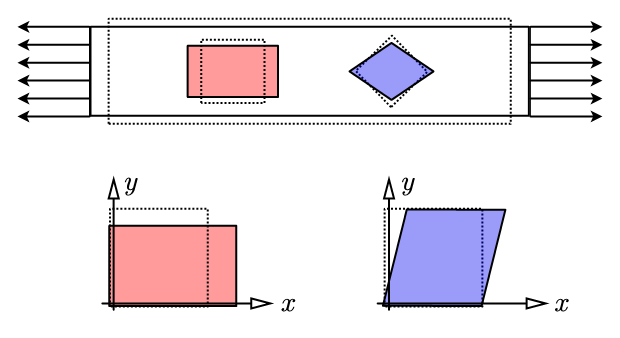
\includegraphics[width=7cm]{image/6-7-1.png}
\caption{正应变与剪应变}\label{6-7-1}
\end{wrapfigure}
其中三个对角元素$\varepsilon$称作\emph{正应变}(normal strain).\,而非对角的元素$\theta$称作\emph{剪应变}(shear strain).\,如图\ref{6-7-1}所示,\,在一种非常简单的模型中,\,大气中的棒被在沿棒方向施加一个拉力而伸长,\,但宽方向很自然地会产生些许的收缩.\,那么根据在棒里取出不同的微元形式,\,其变形方向也会有所改变.\,红色部分沿$x$方向就发生了明显的正应变.\,这是因为合适地平移,\,旋转其变形后的微元对齐形变前的微元(虚线)后,\,明显发现在$x$方向长度变大了.\,如果初始长度为$X$,\,之后在微元范围内端点的$x=X+\delta$.\,于是根据上面的定义,\,正应变其实就是:
\[\varepsilon=\frac{\delta}{X}=\frac{x-X}{X}\]

而蓝色部分是个平行四边形,\,将底边与变形前的底边对齐以后,\,我们发现$x-y$平面上顶角不再是$90^\circ$,\,这其实就标志着剪应变.\,如果这个角度减小了$\alpha$,\,那么之后的$x=X+Y\tan\alpha,\,y=Y$.\,这就说明$\delta_x=Y\tan\alpha,\,\delta_y=0$.\,从而:
\[\theta_{xy}=\frac{\partial \delta_y}{\partial X}+\frac{\partial \delta_x}{\partial Y}=\tan\alpha\approx \alpha\]

可见这个角度变化其实就是剪应变,\,它与边的对齐方式无关,\,如果$x,\,y$轴夹角变小便是正的.\,正应变,\,剪应变都是无量纲的物理量.

\vspace{0.5cm}

接下来需要考虑弹性体的内部受力情况.\,令人惊讶的是,\,它也必然由一个对称张量描述.\,首先我们意识到弹性力内部的受力具有以下特征:\,A.\,是空间点的函数,\,不同点处可以不同,\,但每一点应当有一个受力情况,\,它就是内部的\emph{应力}(stress).\,B.\,不是一个矢量.\,显然指出弹性体中的一点,\,并不能马上对应出来这个点处的某个受力的情况,\,因为我们考虑的是内力而不是外力,\,但是点处的受力不可能有明确的施力物体与受力物体.\,那么其实还需要在这一点处找到一个面矢量$\ud \bs{S}$,\,才能说是谁对谁的力.\,我们这样就发现了,\,其实指定一个应力,\,本质上就是在每一点指定一个面矢量$\ud \bs{S}$到相互作用力$\ud \bs{F}$的映射.\,C.\,显然,\,这样的映射应当为线性映射\footnote{证明留给读者做思考,\,需要用到极限微元受力分析.}.

\begin{wrapfigure}[9]{o}[-10pt]{7cm}
\centering
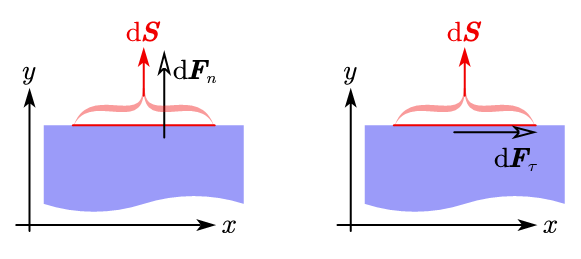
\includegraphics[width=7cm]{image/6-7-2.png}
\caption{正应力与剪应力}\label{6-7-2}
\end{wrapfigure}
这样就几乎已经说明,\,应力其实就是一个张量.\,因为从一个矢量$\ud \bs{S}$到另一个矢量$\ud \bs{F}$的线性映射的数学模型其实就是张量,\,它存在$3\times 3=9$个分量.\,我们进一步指定,\,$\ud \bs{F}$的含义$\ud \bs{S}$指向的那一侧的体元对这一侧的体元通过$\ud \bs{S}$施加的相互作用力.\,这个张量就是:
\[\left\{\begin{array}{ccc}\ud F_x &= & \sigma_{xx} \ud S_x + \sigma_{xy} \ud S_y+\sigma_{xz} \ud S_z \\ \ud F_y&= & \sigma_{yx} \ud S_x + \sigma_{yy} \ud S_y+\sigma_{yz} \ud S_z \\ \ud F_z &= & \sigma_{zx} \ud S_x + \sigma_{zy} \ud S_y+\sigma_{zz} \ud S_z \end{array}\right.\]
\[\bs{\sigma}:\; \ud \bs{S}\rightarrow \ud \bs{F}\]

\[\bs{\sigma}:\; \begin{bmatrix}\sigma_{xx}&\sigma_{xy}&\sigma_{xz}\\\sigma_{yx}&\sigma_{yy}&\sigma_{yz}\\\sigma_{zx}&\sigma_{zy}&\sigma_{zz}\end{bmatrix}\]

这个张量就叫做\emph{应力张量}(stress tensor).\,通过极限微元的受力分析,\,可以证明这个张量还必须是对称的\footnote{也留给读者自己完成.}.\,也就是说,\,我们可以写成以下形式:
\[\bs{\sigma}:\; \begin{bmatrix}\sigma_{x}&\tau_{xy}&\tau_{zx}\\\tau_{xy}&\sigma_{y}&\tau_{yz}\\\tau_{zx}&\tau_{yz}&\sigma_{z}\end{bmatrix}\]

同样的,\,参考图\ref{6-7-2},\,我们可以发现,\,对角线元素$\sigma$代表\emph{正应力}(normal stress)而非对角线元素$\tau$代表\emph{剪应变}(shear stress).\,如果把面元取为$\ud\bs{S}=\ud S_y\bs{e}_y$,\,考虑在平面上的受力就会产生两个分量:
\[\ud \bs{F}_n=\sigma_y \ud S_y\bs{e}_y\quad,\quad\ud \bs{F}_{\tau}=\tau_{xy} \ud S_y\bs{e}_x\]

前者就是垂直于面的以拉力为正的正应力,\,后者就是平行于面方向的剪应力.\,而应力本身都是和以往学过的压强量纲一致,\,国际单位是帕斯卡${\rm Pa}$:
\[\sigma=\frac{\ud F_n}{\ud S}\quad ,\quad \tau=\frac{\ud F_{\tau}}{\ud S}\]

\vspace{0.5cm}

引入两个张量以后,\,剩下的就是构造两者之间的因果关系:\,应力是如何造成应变的.\,在纯粹的弹性理论中,\,我们可以假设应力张量到应变张量的映射再一次是一个逐点线性的映射.\,这样的结果是数学上造成了每一点需要引入一个四阶的张量来描述这样的映射.\,三维情况下四阶的张量一共会造成$3^4=81$个独立分量.\,由于应力应变张量本身具有对称性,\,故其实只需要$6^2$个独立分量.\,再由于体系的非耗散性的要求\footnote{导致了某种形式互易定理.},\,其独立分量数最终减少到$21$个.\,这也是高度非对称的介质的弹性系数中独立的量的个数.\,然而,\,如果介质是完全各向同性的,\,也就是说沿所有三维空间中任意方向的长度与角度的拉伸与压缩都是相同困难的情况下,\,张量的对称性理论可以告诉我们,\,独立的弹性系数只会剩下两个.\,具体来说,\,$\bs{\varepsilon}$与$\bs{\sigma}$之间的关系必然会变成以下不依赖于坐标系选取的形式:
\[\bs{\sigma}=2\mu\cdot\bs{\varepsilon}+\lambda {\rm Tr}(\bs{\varepsilon})\cdot\bs{I}\]

而按照这样的方式选取的弹性系数$\lambda$和$\mu$被叫做\emph{拉梅参数}(Lam\'e parameters).\,式中${\rm Tr}$代表取迹操作,\,而$\bs{I}$是单位张量.\,带入之前的两个张量的写法上式实际上意味着:
\[\sigma_x=2\mu\varepsilon_x+\lambda(\varepsilon_x+\varepsilon_y+\varepsilon_z)\]
\[\sigma_y=2\mu\varepsilon_y+\lambda(\varepsilon_x+\varepsilon_y+\varepsilon_z)\]
\[\sigma_z=2\mu\varepsilon_z+\lambda(\varepsilon_x+\varepsilon_y+\varepsilon_z)\]
\[\tau_{ij}=\mu\theta_{ij}\]

至少我们能从上式发现,\,剪应力和正应力是分别独立地导致剪应变和正应变的,\,尤其是剪应力,\,它在三个方向甚至都是互相独立地,\,而这个比例系数就还被叫做\emph{剪变模量}(shear modulus),\,用$G$来表示.\,即拉梅系数$\mu\equiv G$.\,这个在切向成立的结论称作\emph{横向胡克定律}(transverse Hooke's law):
\[\frac{ F_\tau}{ S}=G \frac{ \delta}{ y}\]

而前三个式子对应的正应力正应变之间的关系比较复杂.\,首先我们把三式相加可以得到:
\[\sigma_x+\sigma_y+\sigma_z=(2\mu+3\lambda)(\varepsilon_x+\varepsilon_y+\varepsilon_z)\]\tabularnewline

我们意识到,\,任何物体在大气环境下实际上就受到周围分子不断撞击产生的大气压力而体积收缩,\,实际上就是三个方向应力相等于压强$\sigma_x=\sigma_y=\sigma_z=p$,\,而且三个应变$\varepsilon_i$就等价于线压缩率,\,应当是体压缩率的三分之一的情况,\,这样我们得到:
\[p=\left(\lambda+\frac{2}{3}\mu\right)\frac{\Delta V}{V}\]

这个系数就叫做\emph{体弹性模量}(bulk modulus):
\[K=\lambda+\frac{2}{3}\mu\]

一般来说,\,弹性体预先在大气体系中被压缩,\,在这个基础上,\,线性地叠加上由于其他形式的应力$\bs{\sigma}$导致的新应变$\bs{\varepsilon}$.\,

还有一种至关重要的变形.\,如果我们在一根弹性棒的$x$方向施加应力$\sigma$,\,但是$y-z$方向不施加任何的力$\sigma_y=\sigma_z=0$,\,扣除原来大气造成的应变,\,通过解方程得到$\varepsilon=\varepsilon_x$和$\varepsilon'=\varepsilon_y=\varepsilon_z$的值:
\[\left\{\begin{array}{ccc}\sigma &=&2\mu\varepsilon + \lambda(\varepsilon+2\varepsilon') \\ 0 &=&2\mu\varepsilon' + \lambda(\varepsilon+2\varepsilon')\end{array}\right.\Rightarrow\quad \left\{\begin{array}{ccc}\varepsilon &=& \frac{\lambda+\mu}{\mu(3\lambda+2\mu)} \sigma\\ \varepsilon' &=&-\frac{\lambda}{2(\lambda+\mu)}\varepsilon\end{array}\right.\]

第一个式子翻过来写就是描述拉力与棒伸长之间的\emph{纵向胡克定律}(longtitudinal Hooke's law).\,相关的弹性系数称作\emph{杨氏模量}(Young's modulus),\,即$E=\mu(3\lambda+2\mu)/(\lambda+\mu)$.\,而第二个式子反映了如果棒在拉力方向伸长,\,在垂直方向必然缩短的现实.\,缩短率与伸长率的比值称为\emph{泊松比}(Poisson's ratio),\,即$nu=\lambda/2(\lambda+\mu)$:
\[\frac{F_n}{S}=E\frac{\delta}{x}\quad ,\quad \frac{\delta'}{y}=\nu\frac{\delta}{x}\]

\begin{figure}[H]
\centering
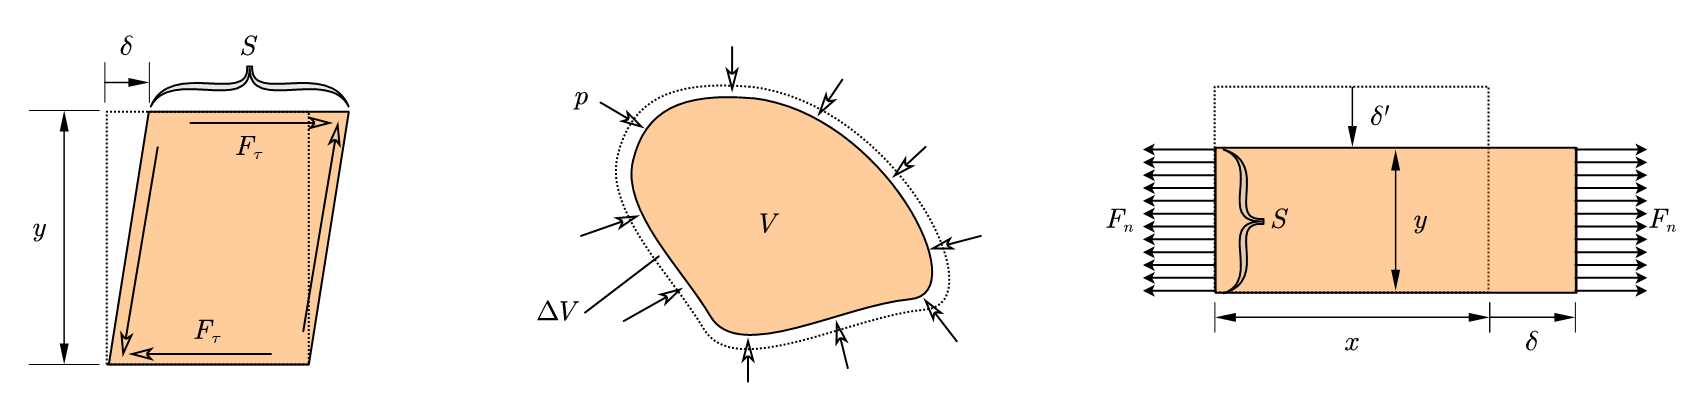
\includegraphics[width=14cm]{image/6-7-3.png}
\caption{剪变模量,\,体弹性模量与杨氏模量}
\end{figure}

三个弹性模量的单位也是应力的单位,\,即帕斯卡,\,而典型材料的弹性模量在$10^{10}{\rm Pa}$的数量级.


\section{弹性棒, 弹性绳, 弹性膜与弹性体}

在弹性的语境下,\,除了体状的大块弹性介质的研究,\,一些边缘化的状态:\,比如弹性体的表面,\,或者本来就在空间上受到限制的情况,\,包括本节介绍的弹性棒,\,绳,\,膜等,\,都是值得研究,\,且具有相似行为的体系.\,这种相似性体现在具有同一类的动力学方程和能量结构上.\,并最终导致了下一节介绍的弹性波的结果.

\subsection{弹性棒}

\begin{wrapfigure}[17]{o}[-10pt]{6cm}
\centering
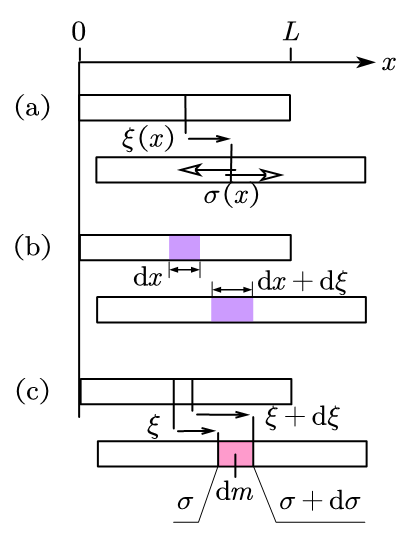
\includegraphics[width=6cm]{image/6-7-4.png}
\caption{弹性棒的建模}\label{6-7-4}
\end{wrapfigure}
考虑一根弹性棒\ref{6-7-4},\,忽略其在垂直棒方向的运动带来的动力学效应.\,那么棒就被简化为一维的模型.\,在变量上,\,我们选取棒未形变时的坐标$x$和时间$t$为自变量,\,而沿正方向向前的位移$\xi$为因变量,\,即$\xi(x,\,t)$.\,此时如(a)图,\,在棒上$x$处找一个固连在棒上的面元,\,随$x$改变的不仅仅是$\xi$,\,其实还有通过这一个面元相互拉扯的应力$\sigma$.\,于是我们就来到了(b)中关于应力的计算.\,同时参考(c)图,\,一个体积元$\ud x$的左右侧原坐标$x$与$x+\ud x$,\,但是它们的位移是不一样的,\,前者是$\xi(x)$,\,后者则是$\xi(x+\ud x)=\xi+\ud \xi$,\,即:
\[\ud \xi=\frac{\partial \xi}{\partial x}\ud x\]

那么这一段微元长度就变为$\ud x+\ud \xi$.\,根据胡克定律,\,由于伸长产生的应力就是:
\[\sigma(x,\,t)=E\frac{\ud \xi}{\ud x}=E\frac{\partial \xi}{\partial x}\]

最后(c)图再取出$\ud x$的微元,\,其质量密度为$\rho$,\,截面积为$S$,\,那么其质量和两段受力的合力为:
\[\ud m=\rho S\ud x\]
\[\ud F=\ud \sigma S=ES\frac{\partial^2 \xi}{\partial x^2}\ud x\]

根据牛顿第二定律$\ud F=\ud m \cdot a$,\,$a$则是位移$u$对时间的二阶导数.\,这就给出了以下方程:
\[\frac{\partial^2 \xi}{\partial t^2}=\frac{E}{\rho} \frac{\partial^2 \xi}{\partial x^2}\]

这样的方程有一个名字,\,这也是我们第一次遇到这样的方程,\,称为\emph{波动方程}(wave equation).\,一维波动方程的一般形式为:
\[\frac{\partial^2 \xi}{\partial t^2}=v^2 \frac{\partial^2 \xi}{\partial x^2}\]

其中$v$必须是一个常数数学上才叫波动方程,\,$v$称为\emph{波速}(wave velocity).\,而弹性棒对应的波速就是:
\[v=\sqrt{\frac{E}{\rho}}\]

波动方程和波速,\,正如其名,\,在下一节我们去解它之后就会发现就是产生的弹性波的特征.

下一个问题是考虑棒振动的能量.\,动能是比较简单的,\,我们把微元的动能做积分就是总动能:
\[T=\int_0^L \frac{1}{2}\ud m \left(\frac{\partial \xi}{\partial t}\right)^2\]

但我们尤其关心能量的\emph{定域化}(localization)问题.\,就是说能量是否可以表示为逐点的能量密度的体积分.\,就动能来看这也是成立的:
\[T=\int_0^L\mathscr{T}\cdot S\ud x\quad\Rightarrow \quad \mathscr{T}=\frac{1}{2}\rho\left(\frac{\partial \xi}{\partial t}\right)^2\]

现在我们来思考势能的定义.\,显然棒不均匀伸长的情况相对于以往棒均匀伸长是两种完全不同的情况,\,棒所储存的势能不仅要重新推导,\,甚至需要在推导中确立其存在性.\,事实上如果某一段$\ud x$内应力为拉力$\sigma>0$,\,那么如果在这个力下这一段伸长$\ud \xi(t+\ud t)-\ud \xi(t)=\frac{\partial }{\partial t}\left(\frac{\partial \xi}{\partial x}\ud x\right)\ud t$,\,内部应力就会做负功,\,我们只需要证明这个功对应的功率(除以$\ud t$)等于对应体积内的势能的增加,\,即:
\[ES\frac{\partial \xi}{\partial x}\cdot \frac{\partial^2 u}{\partial x\partial t}\ud x=\frac{\ud}{\ud t} (\mathscr{V}S\ud x)\]

这样就得到了:
\[\mathscr{V}=\frac{1}{2}E\left(\frac{\partial \xi}{\partial x}\right)^2\quad ,\quad V=\int_0^L\mathscr{V}\cdot S\ud x\]

总能量总是要守恒的,\,对于棒的能量的计算,\,现在就可以普遍地写为棒上\emph{能量密度}(energy density)的积分,\,这个总能量密度就是动能密度$\mathscr{T}$和势能密度$\mathscr{V}$的和:
\[w=\frac{1}{2}\rho\left(\frac{\partial \xi}{\partial t}\right)^2+\frac{1}{2}E\left(\frac{\partial \xi}{\partial x}\right)^2\]

\subsection{弹性绳}
考虑一条质量线密度为$\lambda$,\,预先被拉紧且拉力为$T$的细绳.\,由于形变小所以沿绳方向的拉力几乎是个常数.\,那么考虑这个绳在垂直$x$方向发生位移$\xi(x,\,t),\,\eta(x,\,t)$.\,我们立马就发现了这个问题不同于上一个问题之处在于因变量变多了.\,上一个弹性棒中的运动模式是\emph{纵波}(lontitudinal wave).\,而这里要建立的是垂直传播方向的\emph{横波}(transverse wave)模型.\,横波不同于纵波的一大本质区别在于它有\emph{偏振}(polarization).\,我们把$\xi$和$\eta$两个方向叫做其偏振方向.
\begin{figure}[H]
\centering
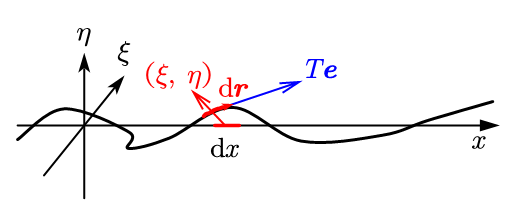
\includegraphics[width=8cm]{image/6-7-5.png}
\caption{弹性绳的建模}
\end{figure}

在建模上,\,两者具有相似性.\,同样是找到$\ud x$微元两端作用的力.\,现在它大小几乎就是$T$,\,只是方向变成了$\bs{e}$,\,它是绳端的单位切向量:
\[\ud\bs{r}=(\ud x,\,\ud \xi,\,\ud \eta)\quad\Rightarrow \quad \bs{e}=\frac{(\ud x,\,\ud \xi,\,\ud \eta)}{\sqrt{\ud x^2+\ud \xi^2+\ud \eta^2}}\]

由于在$\xi,\,\eta$方向的位移产生的斜率是小量,\,上式近似为:
\[\bs{e}=\left(1,\,\frac{\ud \xi}{\ud x},\,\frac{\ud \eta}{\ud x}\right )=\left(1,\,\frac{\partial \xi}{\partial x},\,\frac{\partial \eta}{\partial x}\right )\]

那么拉力$T\bs{e}$的主要效果也就是在$T_\xi=T\frac{\partial \xi}{\partial x}$和$T_\eta=T\frac{\partial \eta}{\partial x}$两个方向上,\,在微元段$\ud x$两侧的力的差产生了在$\xi,\,\eta$方向的加速度.\,那么就得到了波动方程:
\[\frac{\partial^2 \xi}{\partial t^2}=\frac{T}{\lambda} \frac{\partial^2 \xi}{\partial x^2}\]
\[\frac{\partial^2 \eta}{\partial t^2}=\frac{T}{\lambda} \frac{\partial^2 \eta}{\partial x^2}\]

可以发现,\,波动方程的形式相对弹性棒没有本质的变化,\,只不过从一个方程变成了两个独立量要满足的波动方程.\,以及波速公式变成了:
\[v=\sqrt{\frac{T}{\lambda}}\]

能量的表现与推导方法也是类似的.\,唯一的区别是现在的密度指的是线密度.\,可以给出:
\[\mathscr{T}=\frac{1}{2}\lambda\left(\frac{\partial \xi}{\partial t}\right)^2+\frac{1}{2}\lambda\left(\frac{\partial \eta}{\partial t}\right)^2\]
\[\mathscr{V}=\frac{1}{2}T\left(\frac{\partial \xi}{\partial x}\right)^2+\frac{1}{2}T\left(\frac{\partial \eta}{\partial x}\right)^2\]

还有一点值得指出.\,就是在这样的情况下势能还有一种极其简单的等效计算方法,\,就是\emph{表面能}(surface energy)的计算方法,\,体系的势能实际上就是简单地正比于变形之后的总绳长的:
\[V=T\int |\ud \bs{r}|=T\int \sqrt{\ud x^2+\ud \xi^2+\ud \eta^2}=T\int \sqrt{1+\left(\frac{\partial \xi}{\partial x}\right)^2+\left(\frac{\partial \eta}{\partial x}\right)^2}\ud x\]

事实上,\,对上式进行小量近似就可以发现:
\[V=T\int \left[1+\frac{1}{2}\left(\frac{\partial \xi}{\partial x}\right)^2+\frac{1}{2}\left(\frac{\partial \eta}{\partial x}\right)^2\right]\ud x=V_0+\int \mathscr{V}\ud x\]

从而不变拉力绳的势能实际上单纯地正比于绳子被拉长到了多长.\,形成单位长度的绳子需要的能量是完全一致的.

\subsection{弹性膜}

\begin{wrapfigure}[10]{o}[-10pt]{7cm}
\vspace{-0.5cm}
\centering
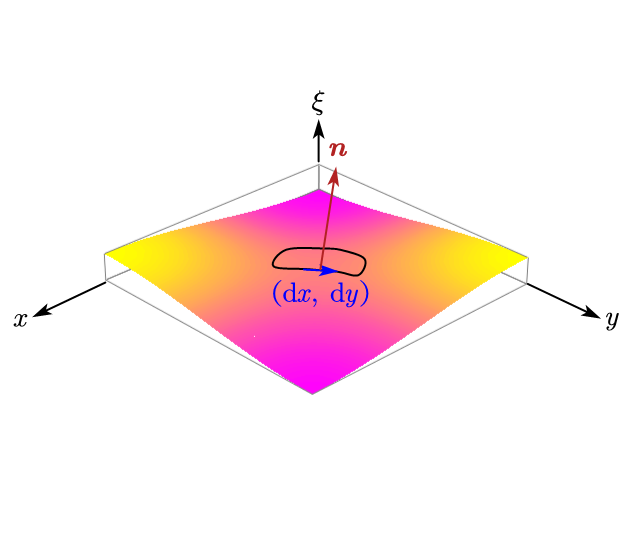
\includegraphics[width=7cm]{image/6-7-6.png}

\vspace{-1.2cm}
\caption{弹性膜的建模}\label{6-7-4}
\end{wrapfigure}

弹性膜的情况则与弹性绳的情况互补:\,这一次是自变量变成了二维的$x,\,y$,\,当然还有时间$t$一共三个.\,倒是因变量只剩下垂直于面方向的位移$\xi$.\,即$\xi(x,\,y,\,t)$.\,面的惯性由质量面密度$\mu$来描述.\,而面的弹性,\,类似于弹性绳,\,我们也给面拉紧造成各向同性的内部张力.\,这种拉紧是均匀的,\,所以才造成均匀的面密度.\,而同时也会对面上线元$\ud s$造成彼此之间垂直于线元的,\,平行于面方向的拉力$\ud F=\sigma \ud s$.\,其中$\sigma$称作\emph{张力系数}(tension coefficient).\,那么如果在$x-y$平面上选取右旋的闭合曲线圈,\,中间围着一块膜.\,在边界上一个典型的线段元和当点处的法向量就是:
\[\ud \bs{r}=(\ud x,\,\ud y,\,\ud \xi)=\left(\ud x,\,\ud y,\,\frac{\partial \xi}{\partial x}\ud x+\frac{\partial \xi}{\partial y}\ud y\right)\quad ,\quad \bs{n}=\left(-\frac{\partial \xi}{\partial x},\,-\frac{\partial \xi}{\partial y},\,1\right)\]

那么通过这一段弧元,\,周围膜对这一段膜施加的力,\,忽略二阶小量就是:
\[\ud \bs{F}=-\sigma\bs{n}\times \ud\bs{r}=\sigma\left(\ud y,\,-\ud x,\,\frac{\partial \xi}{\partial x}\ud y-\frac{\partial \xi}{\partial y}\ud x\right)\]

足以发现,\,如果考虑曲线中的膜受到的合力,\,显然$x-y$方向是平衡的.\,合力在$\xi$方向,\,大小可以根据数学上的格林公式\footnote{\emph{格林公式}(Green formula)为,\,对任何平面区域$D$与其边界右旋闭合曲线$\partial D$:
\[\oint\limits_{\partial D} P(x,\,y)\ud x+Q(x,\,y)\ud y=\iint\limits_D \left(\frac{\partial Q}{\partial x}-\frac{\partial P}{\partial y}\right)\ud x\ud y\]
}得到:
\[F_\xi=\sigma\oint \left(\frac{\partial \xi}{\partial x}\ud y-\frac{\partial \xi}{\partial y}\ud x\right)=\iint \sigma\left(\frac{\partial^2 \xi}{\partial x^2}+\frac{\partial^2 \xi}{\partial y^2}\right)\ud x\ud y\]

从中我们可以发现,\,单位面积上给出的内力就是:
\[f=\frac{\ud F_\xi}{\ud x\ud y}=\sigma\left(\frac{\partial^2 \xi}{\partial x^2}+\frac{\partial^2 \xi}{\partial y^2}\right)\]

那么根据牛顿第二定律,\,这就是让膜产生$\xi$方向加速度的力.\,化简就得到了膜对应的二维波动方程:
\[\frac{\partial^2 \xi}{\partial t^2}=\frac{\sigma}{\mu}\left(\frac{\partial^2 \xi}{\partial x^2}+\frac{\partial^2 \xi}{\partial y^2}\right)\]

对应波速就是:
\[v=\sqrt{\frac{\sigma}{\mu}}\]

同理,\,对应动能和势能的面密度为:
\[\mathscr{T}=\frac{1}{2}\mu\left(\frac{\partial \xi}{\partial t}\right)^2\]
\[\mathscr{V}=\frac{1}{2}\sigma\left(\frac{\partial \xi}{\partial x}\right)^2+\frac{1}{2}\sigma\left(\frac{\partial \xi}{\partial y}\right)^2\]

同样的,\,势能可以重新表述为表面能:
\[V=\sigma\int|\ud \bs{S}|V_0+\int \mathscr{V}\ud x\ud y\]

\subsection{弹性体*}

终于我们可以讨论自变量有$x-y-z$三维空间和$t$一维时间,\,因变量,\,即弹性体的位移矢量$\bs{\delta}$也有三个维度的最复杂的情况.\,本章第一节的讨论总结下来就是两个式子:
\[\bs{\varepsilon}=\frac{1}{2}(\nabla\bs{\delta}+\phantom{}^{\rm t}\nabla\bs{\delta})\]
\[\bs{\sigma}=2\mu\cdot\bs{\varepsilon}+\lambda {\rm Tr}(\bs{\varepsilon})\cdot\bs{I}\]

它给出了位移的一阶倒数是如何产生力的.\,另外一部分物理公式,\,就是计算单位体积受到的合力,\,最后联立牛顿第二定律,\,我们就有希望给出波动方程.

计算合力需要对一个体积区域$D$的边界闭合外向曲面$\partial D$上受到的外力进行积分:
\[\bs{F}=\oint\limits_{\partial D}\ud\bs{S}\cdot\bs{\sigma}\]

这其实可以使用数学上广义上的高斯定理化为体积分:
\[\bs{F}=\iiint\limits_{D}\nabla\cdot\bs{\sigma}\ud x\ud y\ud z\quad\Rightarrow \quad \bs{f}=\frac{\ud\bs{F}}{\ud x\ud y\ud z}=\nabla\cdot\bs{\sigma}\]

最后再联立牛顿第二定律,\,我们就化简出来第三个方程:
\[\frac{\partial^2 \bs{\delta}}{\partial t^2}=\frac{1}{\rho}\nabla\cdot\bs{\sigma}\]

可以得到,\,如果把$\bs{\delta}$记做$(\xi,\,\eta,\,\zeta)$,\,那么对应的方程就称作\emph{纳维-柯西方程}(Navier-Cauchy equation).\,完全展开的形式为:
\[\frac{\partial^2 \xi}{\partial t^2}=\frac{\lambda+2\mu}{\rho}\frac{\partial^2 \xi}{\partial x^2}+\frac{\lambda+\mu}{\rho}\left(\frac{\partial^2 \eta}{\partial x\partial y}+\frac{\partial^2 \zeta}{\partial x\partial z}\right)\]
\[\frac{\partial^2 \eta}{\partial t^2}=\frac{\lambda+2\mu}{\rho}\frac{\partial^2 \xi}{\partial y^2}+\frac{\lambda+\mu}{\rho}\left(\frac{\partial^2 \zeta}{\partial y\partial z}+\frac{\partial^2 \xi}{\partial y\partial x}\right)\]
\[\frac{\partial^2 \zeta}{\partial t^2}=\frac{\lambda+2\mu}{\rho}\frac{\partial^2 \xi}{\partial z^2}+\frac{\lambda+\mu}{\rho}\left(\frac{\partial^2 \xi}{\partial z\partial x}+\frac{\partial^2 \eta}{\partial z\partial y}\right)\]

这样写是不利于我们分析其求解的.\,通过数学化简,\,我们暂时先把波动方程写成如下形式:
\[\rho\frac{\partial^2 \bs{\delta}}{\partial t^2}=(\lambda+2\mu)\nabla(\nabla\cdot \bs{\delta})-\mu\nabla\times(\nabla\times\bs{\delta})\]

其中需要用到矢量微分恒等式:
\[\nabla(\nabla\cdot \bs{\delta})-\nabla\times(\nabla\times\bs{\delta})=\nabla^2\bs{\delta}\]

最后,\,棒中的能量守恒,\,动能密度是简单的.\,而势能密度在只有正应变或剪应变情况下容易证明,\,它就是应力和产生的应变乘积的一半.\,普遍情况下只需要做叠加即可:
\[\mathscr{T}=\frac{1}{2}\rho\left(\frac{\partial \bs{\delta}}{\partial t}\right)^2=\frac{1}{2}\rho\left(\frac{\partial \xi}{\partial t}\right)^2+\frac{1}{2}\rho\left(\frac{\partial \eta}{\partial t}\right)^2+\frac{1}{2}\rho\left(\frac{\partial \zeta}{\partial t}\right)^2\]
\[\mathscr{V}=\frac{1}{2}(\sigma_x\varepsilon_x+\sigma_y\varepsilon_y+\sigma_z\varepsilon_z+\tau_{xy}\theta_{xy}+\tau_{yz}\theta_{yz}+\tau_{zx}\theta_{zx})=\frac{1}{2}\lambda(\nabla\cdot\bs{\delta})^2+\frac{1}{2}\mu(\nabla\bs{\delta}:\nabla\bs{\delta}+\phantom{}^{\rm t}\nabla\bs{\delta}:\nabla\bs{\delta})\]

式中``$:$''符号表示张量之间的双点乘运算.\,具体来说:
\[\left(\sum_{ij}T_{ij}\bs{e}_i\bs{e}_j\right):\left(\sum_{ij}S_{ij}\bs{e}_i\bs{e}_j\right)={\rm Tr}(\bs{T}\cdot\bs{S})=\sum_{ij}T_{ij}S_{ji}\]

\section{弹性波}

波动方程的求解问题其实是非常简单的.\,它其实是普遍的\emph{偏微分方程}(partial differential equation,\,PDE)求解问题中最简单的一类.\,不同于常微分方程,\,一个多元函数,\,如$\xi(x,\,t)$,\,在自变量取某值时不仅仅可以求函数值和对$x$的各阶导数,\,还可以求对$t$的各阶导数,\,甚至还可以求$x$和$t$的各阶混合导数.\,对这些值提出限制,\,就构成了偏微分方程:
\[F\left(x,\,t,\,\frac{\partial^{m+n}\xi}{\partial x^m\partial t^n}\right)=F\left(x,\,t,\,\xi,\,\frac{\partial\xi}{\partial x},\,\frac{\partial\xi}{\partial t},\,\frac{\partial^2\xi}{\partial x^2},\,\frac{\partial^2\xi}{\partial x\partial t}\cdots\right)=0\]

与常微分方程类似的一点是,\,它一般也存在着大量的解.\,尤其是线性偏微分方程的特殊情况,\,其解也是满足常微分方程的叠加原理,\,通特解原理的:
\[\sum_{i,\,j}c_{ij}(x,\,t)\frac{\partial^{m+n}\xi}{\partial x^m\partial t^n}=f(x,\,t)\]

其中最简单的波动方程其实就是二阶的齐次的常系数的线性偏微分方程:
\[f(x,\,t)=0,\,c_{00}=c_{01}=c_{10}=0,\,c_{20}=-v^2,\,c_{11}=0,\,c_{02}=1,\,c_{ij}=0\;(i>2\,{\rm or}\,j>2)\]
\[\Rightarrow\quad \frac{\partial^2 \xi}{\partial t^2}=v^2 \frac{\partial^2 \xi}{\partial x^2}\]

如何找到以上方程的所有解(通解)?\,我们介绍两种常见的思路:

\subsection{分离变量法}

猜测原方程具有如下形式的特解:
\[\xi(x,\,t)=A(x)u(t)\]

代入原方程,\,两边同时除以$A(x)u(t)$,\,化为纯粹的分离变量的常微分方程形式:
\[\frac{\frac{\ud^2 u}{\ud t^2}}{u}=v^2\frac{\frac{\ud^2 A}{\ud x^2}}{A}\]

左侧必然是不含$x$的那一类函数.\,而右侧又必须是不含$t$的那一类函数.\,两者还是同一个函数.\,所以这个函数$x,\,t$都不含有,\,那便是常数.\,最后再注意到随时间变化的部分在简谐函数下恰好能符合常数的要求:
\[u(t)=\ue^{\ui\omega t}\quad \Rightarrow\quad \frac{\frac{\ud^2 u}{\ud t^2}}{u}=-\omega^2\]

最后求解对$A$的限制,\,得到:
\[A(x)=A\ue^{\mp\ui kx}\quad,\quad \frac{\omega}{k}=v\]

从而我们就得到了通解的一组基:
\[\left\{\xi(x,\,t)=A\ue^{\ui(\omega t-kx)},\,\xi(x,\,t)=A\ue^{\ui(\omega t+kx)}\middle|\frac{\omega}{k}=v \right\}\]

根据傅里叶理论.\,上述解的叠加其实就是所有可能在一维下符合波动方程的解.\,这样一组基本的解就是右行波和左行波解.\,注意到这样的波有一点不符合实际情况:\,它完全没有色散,\,所有的频率的波传播速度都完全一样,\,说明我们的建模过于简单.

\subsection{变量代换法}

如果我们尝试变量代换:
\[x_+=x+vt,\,x_-=x-vt\]

那么容易发现,\,原来的方程居然变成了:
\[\frac{\partial^2 \xi}{\partial x_+\partial x_-}=0\]

这样,\,只需要$\xi$仅仅是其中一个变量的函数,\,对另一个函数的偏导数就是零,\,就能符合以上的方程.\,即任意的$f(x_+)$和$g(x_-)$都是以上方程的解.\,由于叠加原理,\,我们就能肯定地找到以下特解:
\[\xi(x,\,t)=g(x-vt)+f(x+vt)\]

这其实也构成了通解,\,它甚至直接就是任意通解的形式,\,不仅仅是可以叠加形成通解的一组基:
\[\left\{\xi(x,\,t)=g(x-vt)+f(x+vt)\middle|\forall f\forall g\right\}\]

其中任意的$g(x-vt)$就代表初始时刻波形$g(x)$任意的一列右行波.\,而$f$就是左行波.\,即任何一维的波动总可以分解为任意波形的左行波和右行波的叠加.\,上一节的任意频率的各种简谐波又可以叠加形成任意波形,\,实际上就是傅里叶理论的重要内容.

\subsection{多维情况}

如果是类似于弹性绳那样的波动方程:
\[\frac{\partial^2 \xi}{\partial t^2}=
v^2 \frac{\partial^2 \xi}{\partial x^2}\quad,\quad \frac{\partial^2 \eta}{\partial t^2}=v^2 \frac{\partial^2 \eta}{\partial x^2}\]

那么这个一维传播的二维振动的基础行波解就可以表达为:
\[(\xi,\,\eta)=(A,\,B)\ue^{\ui(\omega t\pm kx)}\quad,\quad \frac{\omega}{k}=v\]

其中偏振矢量$(A,\,B)$可以是任何可能性,\,如果是$(0,\,1)$就是$\xi$方向的线偏振,\,如果是$(1,\,0)$就是$\eta$方向的线偏振.\,故这个振动还可以按偏振模式分解为两个.\,注意到$A,\,B$都是复数还可以带有相位.\,如果两个方向复振幅的模相等而相位差$90^\circ$,\,那么这个偏振模式就叫做圆偏振.\,即,\,相对简单一维振动,\,它还多了偏振这一个自由度.

\vspace{0.5cm}

如果是类似于弹性膜那样的波动方程:
\[\frac{\partial^2 \xi}{\partial t^2}=v^2\left(\frac{\partial^2 \xi}{\partial x^2}+\frac{\partial^2 \xi}{\partial y^2}\right)\]

那么这个二维传播的一维振动的基础行波解就被表达为:
\[\xi=A\ue^{\ui(\omega t- k_x x-k_y y)}\quad,\quad \frac{\omega}{\sqrt{k_x^2+k_y^2}}=v\]

那么这个波就同时具有了以下自由度:\,频率(决定$\omega$和$k$以及引申的周期,\,波长等等),\,传播方向(决定$k_x$和$k_y$的比例和正负),\,强度(决定$A$的模),\,以及相位(决定$A$的幅角).

\vspace{0.5cm}

最后考虑弹性体中的波动方程,\,即纳维-柯西方程:
\[\rho\frac{\partial^2 \bs{\delta}}{\partial t^2}=(\lambda+2\mu)\nabla(\nabla\cdot \bs{\delta})-\mu\nabla\times(\nabla\times\bs{\delta})\]

这个方程看上去很难直接求解.\,但是实际上数学上有一重要定理为我们提供了重要的线索.\,就是\emph{斯托克斯-亥姆霍兹定理}(Stokes-Helmholtz's theorem)发现,\,任何三维空间中的矢量$\bs{\delta}(\bs{r})$都可以分解为一个有旋无散场$\bs{\delta}_S$与有散无旋场$\bs{\delta}_P$的叠加:
\[\bs{\delta}=\bs{\delta}_S+\bs{\delta}_P\quad :\quad \nabla\cdot \bs{\delta}_S=0\;,\;\nabla \times \bs{\delta}_P=\bs{0}\]

基于这一点,\,我们可以考虑纳维-柯西方程在仅仅有有旋无散的振动和有散无旋的振动情况下的各自的解,\,只要存在,\,叠加在一起就是通解了.\,再次结合式子:
\[\nabla(\nabla\cdot \bs{\delta})-\nabla\times(\nabla\times\bs{\delta})=\nabla^2\bs{\delta}\]

首先考虑有旋无散的振动.\,那么纳维-柯西方程简化为:
\[\rho\frac{\partial^2 \bs{\delta}_S}{\partial t^2}=-\mu\nabla\times(\nabla\times\bs{\delta}_S)\]

但是旋即借助前式发现:
\[-\nabla\times(\nabla\times\bs{\delta}_S)=\nabla^2\bs{\delta}_S\]

这就相当于给出了:
\[\frac{\partial^2 \bs{\delta}_S}{\partial t^2}=v_S^2\nabla^2\bs{\delta}_S=v_S^2\left(\frac{\partial^2 }{\partial x^2}+\frac{\partial^2 }{\partial y^2}+\frac{\partial^2 }{\partial z^2}\right)\bs{\delta}_S\quad ,\quad v_S=\sqrt{\frac{\mu}{\rho}}\]

这样就可以求解了,\,其通解的基为:
\[\bs{\delta}_S=\bs{A}_S\ue^{\ui(\omega t- \bs{k}\cdot\bs{r})}\quad,\quad \frac{\omega}{|\bs{k}|}=v_S\]

最后验证它是否符合散度为零的条件,\,发现必须要满足:
\[\bs{k}\cdot\bs{A}_S=0\quad\Rightarrow\quad \bs{k}\perp\bs{A}_S\]

即这样的波其实是一种横波.\,它构成的要素有频率,\,传播方向,\,强度,\,偏振,\,以及相位.\,这样的弹性体体波称作\emph{剪波}(shear wave).\,它发生的形变就是剪应变,\,其波速恰好用的就是剪边模量$\mu=G$:
\[v_S=\sqrt{\frac{G}{\rho}}\]

再考虑有散无旋的振动.\,那么纳维-柯西方程简化为:
\[\rho\frac{\partial^2 \bs{\delta}_P}{\partial t^2}=(\lambda+2\mu)\nabla(\nabla\cdot \bs{\delta}_P)\]

但是旋即借助前式发现:
\[\nabla(\nabla\cdot \bs{\delta}_P)=\nabla^2\bs{\delta}_P\]

这就相当于给出了:
\[\frac{\partial^2 \bs{\delta}_P}{\partial t^2}=v_P^2\nabla^2\bs{\delta}_P=v_P^2\left(\frac{\partial^2 }{\partial x^2}+\frac{\partial^2 }{\partial y^2}+\frac{\partial^2 }{\partial z^2}\right)\bs{\delta}_P\quad ,\quad v_P=\sqrt{\frac{\lambda+2\mu}{\rho}}\]

这样就可以求解了,\,其通解的基为:
\[\bs{\delta}_P=\bs{A}_P\ue^{\ui(\omega t- \bs{k}\cdot\bs{r})}\quad,\quad \frac{\omega}{|\bs{k}|}=v_P\]

最后验证它是否符合旋度为零的条件,\,发现必须要满足:
\[\bs{k}\times\bs{A}_S=0\quad\Rightarrow\quad \bs{k}//\bs{A}_S\]

即这样的波其实是一种纵波.\,它构成的要素有频率,\,传播方向,\,强度,\,以及相位.\,这样的弹性体体波称作\emph{压波}(pressure wave).\,它发生的形变就是正应变,\,注意其波速用的既不是弹性棒情况的杨氏模量$E$,\,也不是体弹性模量$K$,\,与后者关系更近,\,实际上由第一节的知识:
\[v_P=\sqrt{\frac{K+4G/3}{\rho}}\]

最终我们发现,\,作为纵波的压波波速$v_P$总是要比作为横波的剪波$v_S$快一些.\,故在地震波场合下,\,总是把前者叫做\emph{首波}(primary wave),\,后者叫做\emph{次波}(secondary wave).\,两种命名方法都是导致纵波简记为P波,\,横波简记为S波的原因.\,也经常地,\,我们会把特定方向传播,\,有特定频率(横纵波速不同会导致$k$不同)的横波两种偏振,\,加上纵波称作三种不同的偏振,\,波从振源传播到特定点,\,三种偏振需要的时间是不同的.\,纵波总是先到,\,横波后到.

地球内部结构虽然目前只能从现象去反过来建立模型,\,但比较令人相信的一点是内部存在分层的现象,\,在地表以下约$2891{\rm km}$处存在从固态的地幔到高压``液态''的地核的\emph{古登堡不连续性}(Gutenberg discontinuity).\,作为类似于固态的高压液态,\,在建立模型上十分重要的一点是,\,其剪变模量$G$几乎降低到了$0$.\,这给出了两个结果:\,一是通过剪变的弹性得以传播和存在的剪波无法存在,\,故地震波在地幔-地核分界面上会发生$S$波的全反射\footnote{少量S波有可能转化为P波继续向地核传播}.\,二是压波就彻底变成了由体弹性模量决定的波速公式,\,这一个公式也是正常气体,\,液体中的体波的波速公式:
\[v_P=\sqrt{\frac{K}{\rho}}\]

尤其是在理想气体中,\,比如空气中传播的声波,\,其波速就可以把气体视作理想气体,\,而气团的压缩与膨胀都被视作绝热的(因为振动频率高气体完全无法达到热学平衡),\,于是:
\[pV^\gamma=C\quad\Rightarrow \quad \frac{\ud p}{p}+\gamma\frac{\ud V}{V}=0\]
\[\Rightarrow \quad K=-\frac{\ud p}{\ud V/V}=\gamma p\]

带入声速,\,结合密度公式$\rho=\mu p/RT$,\,得到气体中的声速公式:
\[v=\sqrt{\frac{\gamma RT}{\mu}}\]

这个计算早在1687年就由牛顿完成,\,但是受限于当时几乎等于空白的热学,\,力学理论的限制与同样几乎是空白的实验测量数据,\,牛顿给出的公式中没有出现绝热指数$\gamma$,\,导致它计算出的室温下空气中声速只有$300{\rm m/s}$.\,比正确值$340{\rm m/s}$小了不少.\,这个误差后来由拉普拉斯解释与修正.

%\subsection{再论格波}